\documentclass[aspectratio=1610,12pt,notheorems]{beamer}

\usepackage[utf8x]{inputenc} \usepackage[russian]{babel}
\usepackage{amsmath,amssymb,amsthm,mathtools}
\usepackage{graphicx,caption,subcaption}
\usepackage{hyperref,natbib}
\usepackage{tikz,xcolor}
\usepackage{algorithm,algpseudocode}
\usepackage{makecell}

\usetikzlibrary{arrows,backgrounds,patterns,%
	matrix,shapes,fit,calc,shadows,plotmarks,snakes}

\theoremstyle{plain}
\newtheorem{theorem}{Теорема}
\newtheorem{lemma}[theorem]{Лемма}

\theoremstyle{definition}
\newtheorem{definition}{Определение}
\newtheorem{problem}{Задача}

\usetheme[height=0.97cm]{Rochester}
\usecolortheme{dolphin}

\definecolor{hard}{RGB}{140,50,50}
\definecolor{mnsgold}{RGB}{240,230,200}

\setbeamercolor{headline}{bg=hard,fg=mnsgold}
\setbeamercolor*{frametitle}{parent=headline}

\setbeamercolor{structure}{fg=hard}
\setbeamercolor{subsection in head/foot}{bg=white,fg=hard}
\setbeamercolor{section in head/foot}{bg=hard,fg=mnsgold}
\setbeamercolor{block title}{bg=hard,fg=mnsgold}

\setbeamertemplate{navigation symbols}{}

\def\mitem{\medskip\item}
\def\ps{\\ [0.65cm]} \linespread{1.16}
\def\usl#1#2{\begin{block}{#1} #2 \end{block} \medskip\pause}

\def\ll{\left(} \def\rr{\right)}
\def\lag{\left\langle} \def\rag{\right\rangle}

\title[Mathnonstop 2019: the seminar]
    {\bfseries Математика НОН-СТОП: \\
	Новое в 2019 году}

\author[\ ]
	{Б. А. Золотов,\qquad Д. Г. Штукенберг \\ \vspace{0.3cm}
		{\small Фонд «Время Науки»}}

\institute[\ ]{\ }

\date{10 декабря 2019}

%%%%%%%%%%%%%%
%%%%%%%%%%%%%%

\begin{document}

\frame{\titlepage}

\begin{frame} \begin{center}
	{\small\ } \\ [0.7cm]
	{\Large К чему фотографировать презентацию,\smallskip\\ когда можно её скачать} \\ [0.9cm]
	{\small Слайды доступны по ссылке: \url{http://bit.ly/mns-seminar-11dec2019}}
\end{center} \end{frame}

\begin{frame}
\frametitle{Конструктивные задачи}
	Мы всё так же горячо любим задачи на приведение примера. Они наглядные и незамысловатые, при этом могут быть крайне разнообразными. \ps
	
	Разберём несколько таких задач — от более простых к более сложным.
\end{frame}

\begin{frame}
\frametitle{Простые, но не простые-простые}

\usl{7 класс, 9A–B}{Докажите, что для любого $n$ существует натуральное число $N\!$, у которого ровно $n$ различных натуральных делителей.} \vspace{4mm}

В пункте {\bf A} было $n=43$. А ответ —\pause $$N = 2^{n-1}.$$
\end{frame}

\begin{frame}
\frametitle{Аксиомы выборов}

\usl{7 класс, 3A}{На предприятии работают 50 человек, и они выбирают себе начальника. Есть две кандидатуры, Ваня и Даня. Про каждого работника известно заранее, кому он отдаёт предпочтение: 20 человек за Даню, 30 человек за Ваню. \smallskip \\
Голосование проходит по двухтуровой системе: люди делятся на 5 групп по 10 человек, в каждой группе выбирается кандидат, наиболее популярный среди членов этой группы, и затем из 5 ответов выбирается имя, названное большее число раз. \smallskip \\
Разделите работников на группы так, чтобы в большинстве групп выбрали Даню и он победил на выборах, несмотря на изначально меньшее число голосующих за него.}
\end{frame}

\begin{frame}
\frametitle{Аксиомы выборов}

\begin{center} \tikz{
\begin{scope}[rotate=90,scale=1.2]
	\filldraw[fill=gray,draw=gray,opacity=0.32] (0,0) rectangle (1,5);
	\foreach \x in {0,2,5} {\draw[thick, color=gray]
		(0.5 * \x cm, 0) -- (0.5 * \x cm, 5);}
	\foreach \x in {0,10} {\draw[thick, color=gray]
		(0, 0.5 * \x cm) -- (2.5, 0.5 * \x cm);}
	\foreach \x in {1,3,4} {\draw[color=gray, opacity=0.38]
		(0.5 * \x cm, 0) -- (0.5 * \x cm, 5);}
	\foreach \x in {1,...,9} {\draw[color=gray, opacity=0.38]
		(0, 0.5 * \x cm) -- (2.5, 0.5 * \x cm);}

	\draw (0.5,-0.25) node[right]{\large За Даню};
	\draw (1.75,-0.25) node[right]{\large За Ваню};

	\pause
	\begin{scope} [xscale=-1, xshift=-2.5cm]
	\draw[very thick] (0.5,0) -- (0.5,5);
	\draw[very thick] (2.5,1.5) -- ++ (-1,0) --
		++ (0,0.5) -- ++ (-0.5,0) -- ++(0,-2);
	\draw[very thick] (2.5,3.5) -- ++ (-1,0) --
		++ (0,-0.5) -- ++ (-0.5,0) -- ++(0,2);
	\draw[very thick] (2.5,3.5) --
		++ (-1,0) -- ++ (0,-0.5) --
		++ (-0.5,0) -- ++ (0,-1) -- ++ (0.5,0) --
		++ (0,-0.5) -- ++(1,0);
	\end{scope}
\end{scope} } \end{center} \end{frame}

\begin{frame}
\frametitle{Лабиринт}

\usl{7 класс, 8C}{
Путник в лабиринте видит ситуацию вокруг. Помимо этого, никакой другой 
информации и памяти у него нет. Существует ли какой-нибудь набор правил, чтобы он, 
имея только эту информацию, мог дойти до финальной клетки в любом лабиринте?} \vspace{4mm}

Заметим, что поведение путника однозначно определено в простых ситуациях:

\begin{center} \tikz[scale=0.8]{\begin{scope}[xshift=-3cm]
	\fill[pattern=north east lines] (0,0) -- (0,1) -- (1,1) -- (1,0) -- (1.7,0) -- (1.7,1.7) -- (-0.7,1.7) -- (-0.7,0) -- cycle;
	\draw (0,0) -- (0,1) -- (1,1) -- (1,0);
	\filldraw (0.5,0.5) circle[radius=1.2mm]; \end{scope}
\begin{scope}[xshift=2cm]
	\fill[pattern=north east lines] (-0.7,-0.2) rectangle (0,1.2) (1,-0.2) rectangle (1.7,1.2);
	\draw (0,-0.2) -- (0,1.2) (1,-0.2) -- (1,1.2);
	\filldraw (0.5,0.5) circle[radius=1.2mm];
\end{scope}} \end{center}
\end{frame}

\begin{frame}
\frametitle{Лабиринт}

Приведём решение без $T$-образных перекрёстков, чтобы о них не думать: \pause

\begin{center} \tikz[scale=1.14]{
	\draw (-3,0) ++(0.15,0.15) rectangle ++(5.7,3.7);
	\foreach \x in {-3,...,2} {
	    \foreach \y in {0,...,3} {
		\draw[pattern=north east lines] (\x, \y) ++(0.15,0.15) --
		    ++(0,0.7) -- ++(0.7,0) -- ++(0,-0.7) -- ++(-0.7,0);
	    };
	};
	\draw (2,3.65) node{\itshape\footnotesize Ф};
	\filldraw (0,1.5) circle[radius=0.56mm];
} \end{center} \end{frame}
\begin{frame}
\frametitle{{\itshape Много} примеров}
	Мы попробовали просить участников привести {\itshape как можно больше} способов сделать что-либо — чем больше привёл, тем выше оценка. Порой точное возможное количество способов было не известно даже нам.	
\end{frame}

\def\dwtc{\draw[very thick] }
\def\dtc{\draw[thick] }
\def\dtcg{\draw[thick,color=gray,opacity=0.68] }
\def\dcw{\draw[color=white] }

\def\hexnhex#1{\tikz[scale=0.73]{
    \dcw (-0.3,1) rectangle (0,2); \dcw (3,1) rectangle (3.3,2);
    \foreach \x in {1,...,5} {
	\draw[color=gray, opacity=0.38] (0, 0.5 * \x cm) -- (3, 0.5 * \x cm);
	\draw[color=gray, opacity=0.38] (0.5 * \x cm, 0) -- (0.5 * \x cm, 3);
    }
    \dtc (0,0) -- (0,3) -- (3,3) -- (3,0) -- cycle;
    \dtc #1;
}}

\def\kra{-- ++(0,-0.5) -- ++(-0.5,0) -- ++(0,-0.5) -- ++(0.5,0)}
\def\krb{-- ++(0,-0.5) -- ++(0.5,0) -- ++(0,-0.5) -- ++(-0.5,0)}
\def\tabrow#1{\begin{center}\begin{tabular}{ccc} #1 \end{tabular}\end{center}}

\begin{frame}
\frametitle{Разрезай и властвуй}
\usl{7 класс, 6C}{Предложите как можно больше разных способов разрезать квадрат $6 \times 6$ на два одинаковых многоугольника по линиям сетки.} \vspace{3mm}

\tabrow{
	\hexnhex{(1.5,0) -- (1.5,3)} &
	\hexnhex{(1,0) -- (1,1.5) -- (2,1.5) -- (2,3)} &
	\hexnhex{(0.5,0) -- (0.5,1.5) -- (2.5,1.5) -- (2.5,3)}}
\end{frame}

\begin{frame} \frametitle{Разрезай и властвуй}
\tabrow{
	\hexnhex{(1,0) -- (1,1) -- (1.5,1) -- (1.5,2) -- (2,2) -- (2,3)} &
	\hexnhex{(0.5,0) -- (0.5,1) -- (1.5,1) -- (1.5,2) -- (2.5,2) -- (2.5,3)} &
	\hexnhex{(0.5,3) -- (0.5,1) -- (1.5,1) -- (1.5,2) -- (2.5,2) -- (2.5,0)}}
\tabrow{
	\hexnhex{(1,3) -- (1,0.5) -- (1.5,0.5) -- (1.5,2.5) -- (2,2.5) -- (2,0)} &
	\hexnhex{(1,3) \kra \kra -- (1,0.5) -- (1.5,0.5)
	    -- (1.5,2.5) -- (2,2.5) \krb \krb -- (2,0)} &	
	\hexnhex{(1,3) -- (1,1) -- (1.5,1) -- (1.5,2) -- (2,2) -- (2,0)}}
\tabrow{
	\hexnhex{(1,3) -- (1,1) -- (0.5,1) -- (0.5,0.5) -- (1.5,0.5)
	    -- (1.5,2.5) -- (2.5,2.5) -- (2.5,2) -- (2,2) -- (2,0)} &
	\hexnhex{(0,0.5) -- (2.5,0.5) -- (2.5,2) -- (1,2) -- (1,1.5)
	    -- (2,1.5) -- (2,1) -- (0.5,1) -- (0.5,2.5) -- (3,2.5)} &
	\hexnhex{(0.5,0) -- ++(0,1.5) -- ++(0.5,0) -- ++(0,1) -- ++(0.5,0) -- ++(0,-2)
	    -- ++(0.5,0) -- ++(0,1) -- ++(0.5,0) -- ++(0,1.5)}}
\end{frame}

\begin{frame} \frametitle{Розеттский камень}
\usl{6 класс, 8A}{Перечислите как можно больше пар букв русского языка таких, 
	что если написать эти буквы одна поверх другой, то их будет невозможно
	идентифицировать. Например, совершенно очевидно, что первая пара
	букв ниже — это А и Т, но про вторую пару не понятно, это В и Ь
	или Р и Ь. \def\dvt{\draw[very thick]}
\begin{center}
\begin{tabular}{ccc}
\tikz[scale=0.48]{
	\draw (0,-0.8) node{(1)};
	\dvt (-0.6,0) -- (0,2) -- (0.6,0);
	\dvt (0,0) -- (0,2); \dvt (-0.6,2) -- (0.6,2);
	\dvt (-0.33,0.9) -- (0.33,0.9);
}
& \hspace{0.8in} &
\tikz[scale=0.48]{
	\draw (0.6,-0.8) node{(2)};
	\dvt (0,0) -- (0,2);
	\dvt (0,0) -- (0.6,0); \dvt (0,1) -- (0.6,1); \dvt (0,2) -- (0.6,2);
	\dvt (0.6,0) arc (-90:90:0.5) arc (-90:90:0.5);
}
\end{tabular}
\end{center} \vspace{-0.4cm}} \vspace{4mm}

Понятно, что ВЬ, РЬ, ВР — это одно и то же. А что ещё?
\end{frame}

\begin{frame} \frametitle{Розеттский камень}

\begin{tabular}{lc}
\makecell[l]{
	Интересно попробовать формализовать \\
	данную задачу — понять, что значит \\
	написать букву.\pause \\ [0.35cm]
	Рассмотрим {\itshape 16-сегментный индикатор:} \\
	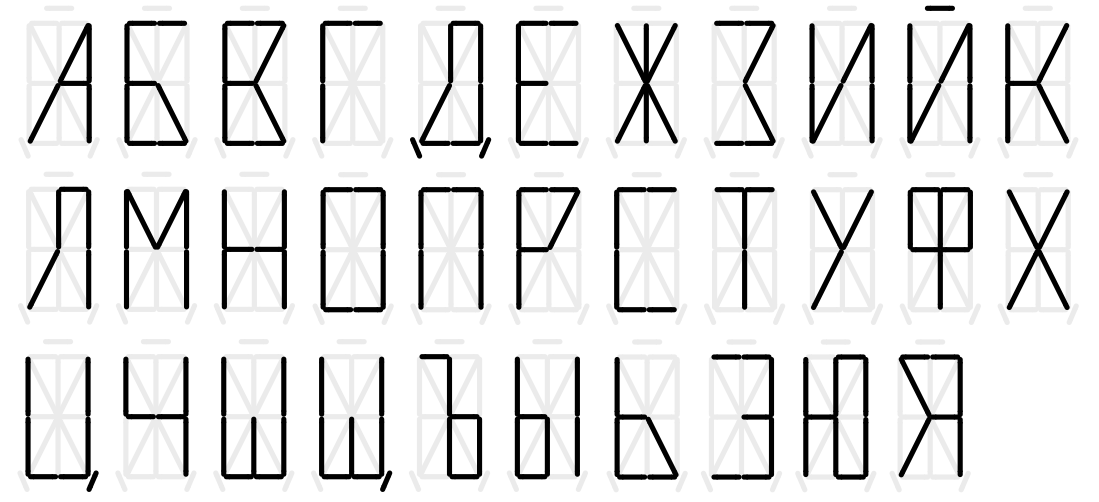
\includegraphics[width=6.2cm]{img/16seg} \pause \\ [0.25cm]
	Вспомним замеченное нами совпадение: \\
\begin{tabular}{ll}
\makecell[l]{{\footnotesize ЬР ЬЗ ЬВ СК СВ РЗ РВ РБ КЗ} \\
{\footnotesize КЕ КВ КБ ЗЕ ЗВ ЗБ ЕВ ГВ ВБ}} &
\makecell[l]{\tikz[scale=0.2]{
  \draw[thick] (-1.000000,2.000000) -- (-1.000000,0.000000);
  \draw[thick] (-1.000000,0.000000) -- (0.000000,0.000000);
  \draw[thick] (-1.000000,-2.000000) -- (-1.000000,0.000000);
  \draw[thick] (1.000000,-2.000000) -- (0.000000,0.000000);
  \draw[thick] (-1.000000,-2.000000) -- (0.000000,-2.000000);
  \draw[thick] (0.000000,-2.000000) -- (1.000000,-2.000000);
  \draw[thick] (-1.000000,2.000000) -- (0.000000,2.000000);
  \draw[thick] (0.000000,2.000000) -- (1.000000,2.000000);
  \draw[thick] (1.000000,2.000000) -- (0.000000,0.000000);
}}
\end{tabular}} & \pause \makecell[c]{
\includegraphics[width=6.5cm]{img/allex}}
\end{tabular} \end{frame}
\begin{frame} \frametitle{Сложные задачи}
	На «Математике НОН-СТОП» мы, разумеется, предлагаем задачи и для детей с некоторым опытом занятия в математических кружках — таким участникам также не будет скучно.
\end{frame}

\begin{frame} \frametitle{Девяносто десять}
\usl{7 класс, 4C}{Кого больше в двоичной записи чисел от 0 до $2^n - 1$ — единиц или нулей? Ответ объясните.} \vspace{4mm}

Нужно придумать однозначное соответствие между единицами \\
и нулями, в котором участвуют все нули, но не все единицы. \\
Но можно проще и изящнее: \ps

	Рассмотрим все возможные
	комбинации из $n$ нулей или единиц. В их записи, очевидно,
	встретится равное количество единиц и нулей. Чтобы получить
	записи чисел, отбросим все ведущие нули.
\end{frame}

\begin{frame} \frametitle{Карфаген\quad{\it\normalsize (Широкий не значит высокий)}}
\usl{8 класс, 1C}{Докажите, что максимальная возможная площадь $n$-угольника, все стороны которого имеют длину 1, меньше, чем максимальная возможная площадь $n+1$-угольника, все стороны которого имеют длину 1.} \vspace{4mm}

Дети же не знают, что максимальную площадь имеют \\
правильные $n$-угольники. \ps

Для каждого многоугольника с $n$ сторонами длины 1 построим многоугольник с $n+1$ сторонами, площадь которого больше.
\end{frame}

\begin{frame} \frametitle{Карфаген\quad{\it\normalsize (Широкий не значит высокий)}}

\begin{center}
\begin{tabular}{ccc}
Если выпуклый & & Если невыпуклый \\
\makecell[c]{
	\definecolor{carthfill}{RGB}{223,223,223}
	\tikz[scale=0.48]{
		\draw[thick] (-1,0) -- ++(60:2) -- (1,0) -- cycle;
		\filldraw[thick,fill=carthfill] (-1,0) ++(195:2) ++(210:2) --
		    ++(30:2) -- ++(15:2) -- ++(0:2) --
		    ++(-15:2) -- ++(-30:2);}
} & \hspace{0.6cm} &
\makecell[c]{
	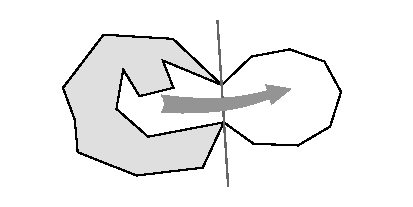
\includegraphics[scale=1.12]{img/carthage}
}
\end{tabular}\end{center}
\end{frame}

\begin{frame} \frametitle{Меняем правила под себя}

Рассмотрим следующую задачу, формулирующуюся \\
самым классическим образом: \medskip

\usl{8 класс, 10C}{В кучке $N$ камней. За ход из неё можно вынуть \vspace{-4mm}
	$$1,\ 2,\ 3,\ \ldots,\ a-1,\ \not{\!a},\ a+1,\ \ldots,\ n\text{\quad камней.}$$
	(То есть любое число от 1 до $n$, кроме $a$.) Играют двое, и про-\linebreak
	игрывает тот, кто не может сделать ход. Кто выиграет при правильной
	игре (в зависимости от чисел $N$, $n$, $a$)?}

Задача решается методом {\it анализа позиций:} не бывает ходов из проигрышной позиции в проигрышную.
\end{frame}
\begin{frame}
\frametitle{Чтение и {\it изменение} авторского условия}
	Мы уже давали задачи, значительная часть решения которых заключалась в их вдумчивом прочтении. \ps
	
	Теперь мы пошли дальше и предложили участникам скорректировать наши условия. Для этого по сути нужно решить задачу «задом наперёд».
\end{frame}

\begin{frame}
\frametitle{Велопоход — 2019}

\usl{7 класс, 10B}{
В августе Саар планирует доехать от Бишкека до Астаны. Она проехала уже
1210 километров. Сверившись с картой, она поняла, что ей осталось ехать втрое
больше, чем расстояние, которое проедет машина, в 4 раза более быстрая, чем Саар,
за время от текущего момента до момента, когда Саар останется столько же,
сколько она проехала сейчас. \smallskip \\
Каково расстояние между Бишкеком и Астаной?}

Пусть осталось ехать $t$\,км. До момента, когда останется 1210, $t-1210$\,км.
\vspace{-3mm}

$$t = 3 \cdot 4 \cdot (t - 1210),\qquad 11t = 12 \cdot 1210,\qquad t = 1320.$$ \vspace{-12mm}

$$1320+1210 = 2530.$$
\end{frame}

\begin{frame}
\frametitle{Велопоход — 2019}

\usl{7 класс, 10C}{
Замените числа 1210 и 4 в условии пункта {\bfseries B} на какие-то другие так,
чтобы ответ в задаче составил 1400 километров — настоящее расстояние между
Бишкеком и Астаной.}

$A$ — сколько уже проехали, $c$ — отношение скоростей машины и велосипеда. \vspace{-5mm}

\begin{align*}
& t = 3c \cdot (t-A),\qquad t = \frac{3cA}{3c-1}. \\
& A + t = A + \frac{3cA}{3c-1} = A \cdot \frac{6c-1}{3c-1}\quad = 1400.
\end{align*}

Например, $A=100$, $c = \frac{13}{36}$.
\end{frame}
\begin{frame}
\frametitle{Ещё проще, ещё доступнее}
	«Математика НОН-СТОП» — олимпиада для всех, и любой участник найдёт в ней то, что сможет решить. \ps

	Разберём несколько задач, доступных каждому.
\end{frame}

\begin{frame}
\frametitle{Конференция анонимных геометров}

\usl{5 класс, 1A}{В комнату, имеющую форму правильного 12-угольника, заходят 124 любителя вычислительной геометрии. Как рассадить их вдоль стен этой комнаты так, чтобы у каждой стены сидело ровно по 11 любителей вычислительной геометрии? \smallskip \\	
	Любителей геометрии можно сажать и в углы комнаты — но не более чем по одному геометру на угол.}
	\vspace{4mm}

$12 \cdot 11 - 124 = 8$. Значит, что в какие-то 8 углов из 12 надо будет посадить геометров.
\end{frame}

\begin{frame}
\frametitle{Незакрученный удар}

\usl{4 класс, 2A}{Шарик катается
по прямоугольнику, не замедляясь. Когда он подъезжает к краю
прямоугольника, он отскакивает от него и продолжает движение.
В каком положении окажется шарик, будучи запущенным
из центра прямоугольника на рисунке, после того как он проедет
24 клетки по диагонали?}

\def\ballandthick{
	\filldraw (0,0) circle[radius=1.2mm];
	\draw[very thick,->] (0,0) -- (-0.72,0.72);
	\draw[very thick] (-1,-1.5) rectangle (1,1.5);
}

\begin{center} \tikz[scale=1.04]{
	\draw (-1.2,0) node[left]{\small \begin{minipage}{4.2cm}\ \end{minipage}};
	\foreach \x in {-2,...,2} {\draw[color=gray] (-0.5 * \x cm, -1.5) -- (-0.5 * \x cm, 1.5);}
	\foreach \x in {-3,...,3} {\draw[color=gray] (-1, -0.5 * \x cm) -- (1, -0.5 * \x cm);}
	\draw[color=gray, thick, dotted] (0,0) -- (-1,1) -- (-0.5,1.5) -- (0.3,0.7);
	\ballandthick;
\pause
	\draw[color=gray, thick, dotted] (0.3,0.7) -- (1,0) -- (-0.5,-1.5) -- (-1,-1) -- (1,1)
	    -- (0.5,1.5) -- (-1,0) -- (0.5,-1.5) -- (1,-1) -- (0,0);
	\ballandthick; \draw[thick] (-1,0) -- (1,0);
	\draw (1.35,0) node[right]{\small \begin{minipage}{5.6cm} Раз в 6 клеток пересекает \\
	    горизонтальную среднюю линию \end{minipage}};
} \end{center} \end{frame}

\begin{frame}
\frametitle{Мы едем, едем, едем, едем, едем, едем...}

\usl{5 класс, 6A}{Проездной на месяц позволяет его владельцу ездить на метро неограниченное число раз, 
стоимость проездного фиксирована и одинакова в любом
месяце. Укажите, какова должна быть стоимость проездного, чтобы при двух ежедневных 
поездках он не окупался бы в феврале, но окупался бы в октябре?
Стоимость разовой поездки в метро равна 45 рублям.}

Октябрь длиннее февраля, поэтому может быть совершено больше поездок. Проездной, таким образом, может быть дешевле стоимости 62 поездок, но дороже стоимости 56 поездок. \vspace{-3mm}

$$28 \cdot 45 \cdot 2 = 2520 < S < 2790 = 31 \cdot 45 \cdot 2.$$
\end{frame}

\begin{frame} \begin{center} \begin{tabular}{ccc}
\makecell[c]{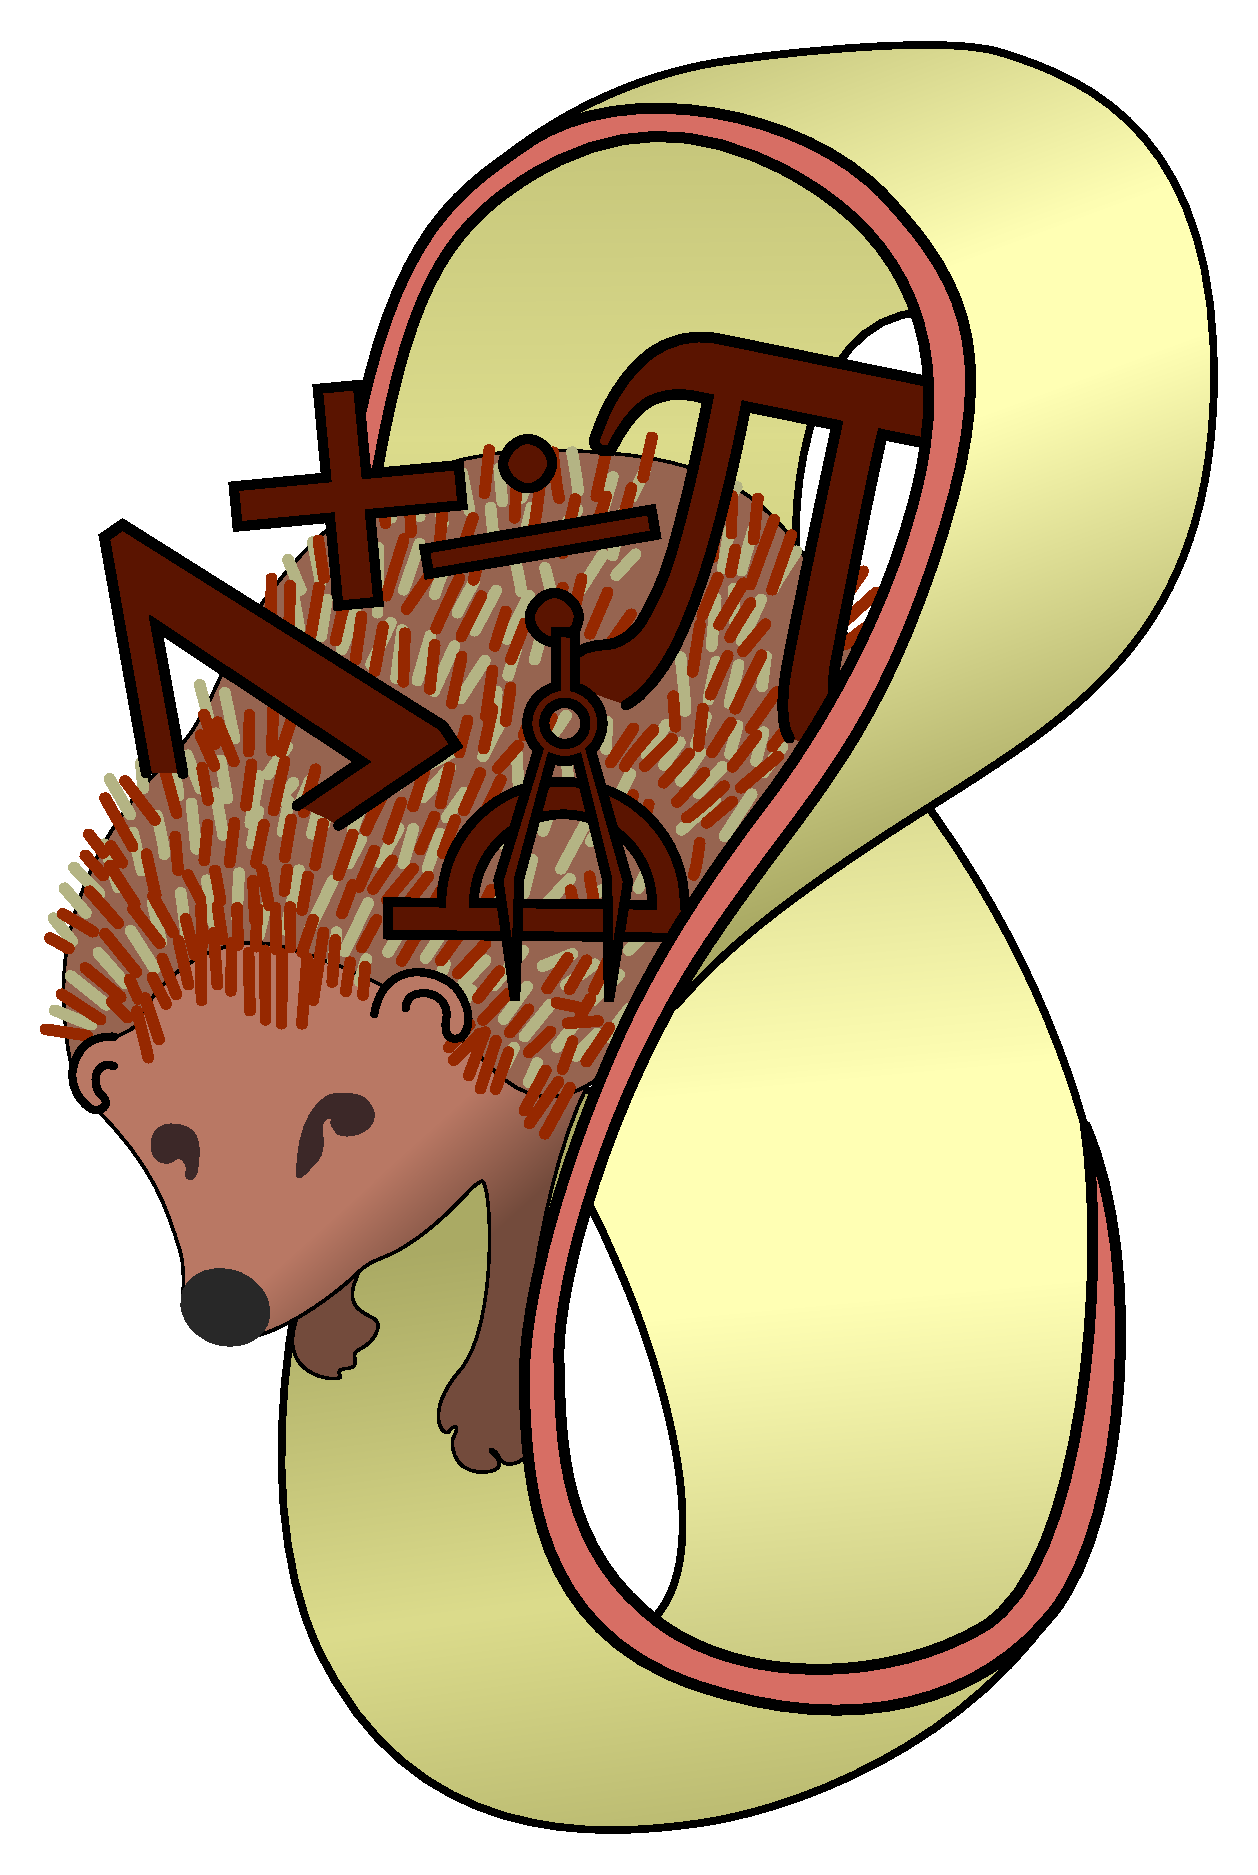
\includegraphics[width=2.2cm]{img/hedgehog}} & &
\makecell[c]{
\includegraphics[width=2.3cm]{img/tsf}} \\
 &	\Huge{Спасибо за внимание!}
\end{tabular} \ps
	\small{Фонд «Время Науки», 2019}
\end{center} \vspace{1.8cm} \end{frame}

\end{document}